\documentclass[a4paper,11pt]{article}
\usepackage[vmargin=1.5cm, hmargin=1.2cm]{geometry}
\usepackage{fontawesome5}
\usepackage[utf8]{inputenc}
\usepackage[T2A]{fontenc}
\usepackage[english, russian]{babel}
\usepackage{datetime}
\usepackage[usenames,dvipsnames]{xcolor}
\usepackage[colorlinks=true, urlcolor=ColorTwo]{hyperref}
\usepackage{tikz}
\usepackage{setspace}
\usepackage{graphicx}
\usepackage{enumitem}
\usepackage{sectsty}
\usepackage{multicol}
\usepackage{adjustbox}
\usepackage{array}
\usepackage{ragged2e}

%---Theme---
\pagenumbering{gobble}
\renewcommand{\baselinestretch}{1.5}
\setlength{\parindent}{0pt}

% Color theme
\definecolor{ColorOne}{RGB}{0,110,140} 	% Blue
\definecolor{ColorTwo}{RGB}{120,0,120} 	% Mauve
\definecolor{ColorThree}{RGB}{140,100,0}% Gold

\sectionfont{\color{ColorOne}}
\subsectionfont{\color{ColorOne}}

% Vertical line
\newcommand{\MyVerticalRule}{%
	\textcolor{ColorOne}{\rule{1pt}{\textheight}}
}

% Update
\newcommand{\LastUpdate}{%
\vfill
\centering \small
\textcolor{ColorOne}{Last updated: \monthname,~\the\year.}
}

% Skip
\newcommand{\MySkip}{
\vskip10pt
}

% Format hyperrefs
\newcommand{\myhref}[2]{%
\href{#1}{\textcolor{ColorTwo}{#2}}
}

% Format skill bullets
\newcommand{\SkillBull}[1]{%
\textcolor{ColorTwo}{#1}
}

\begin{document}
\thispagestyle{empty}

% Left column
\begin{adjustbox}{valign=t}
\begin{minipage}{0.3\textwidth}

\begin{center}
\begin{tikzpicture}
    \clip (0,0) circle (2cm);
    \node at (0,0) {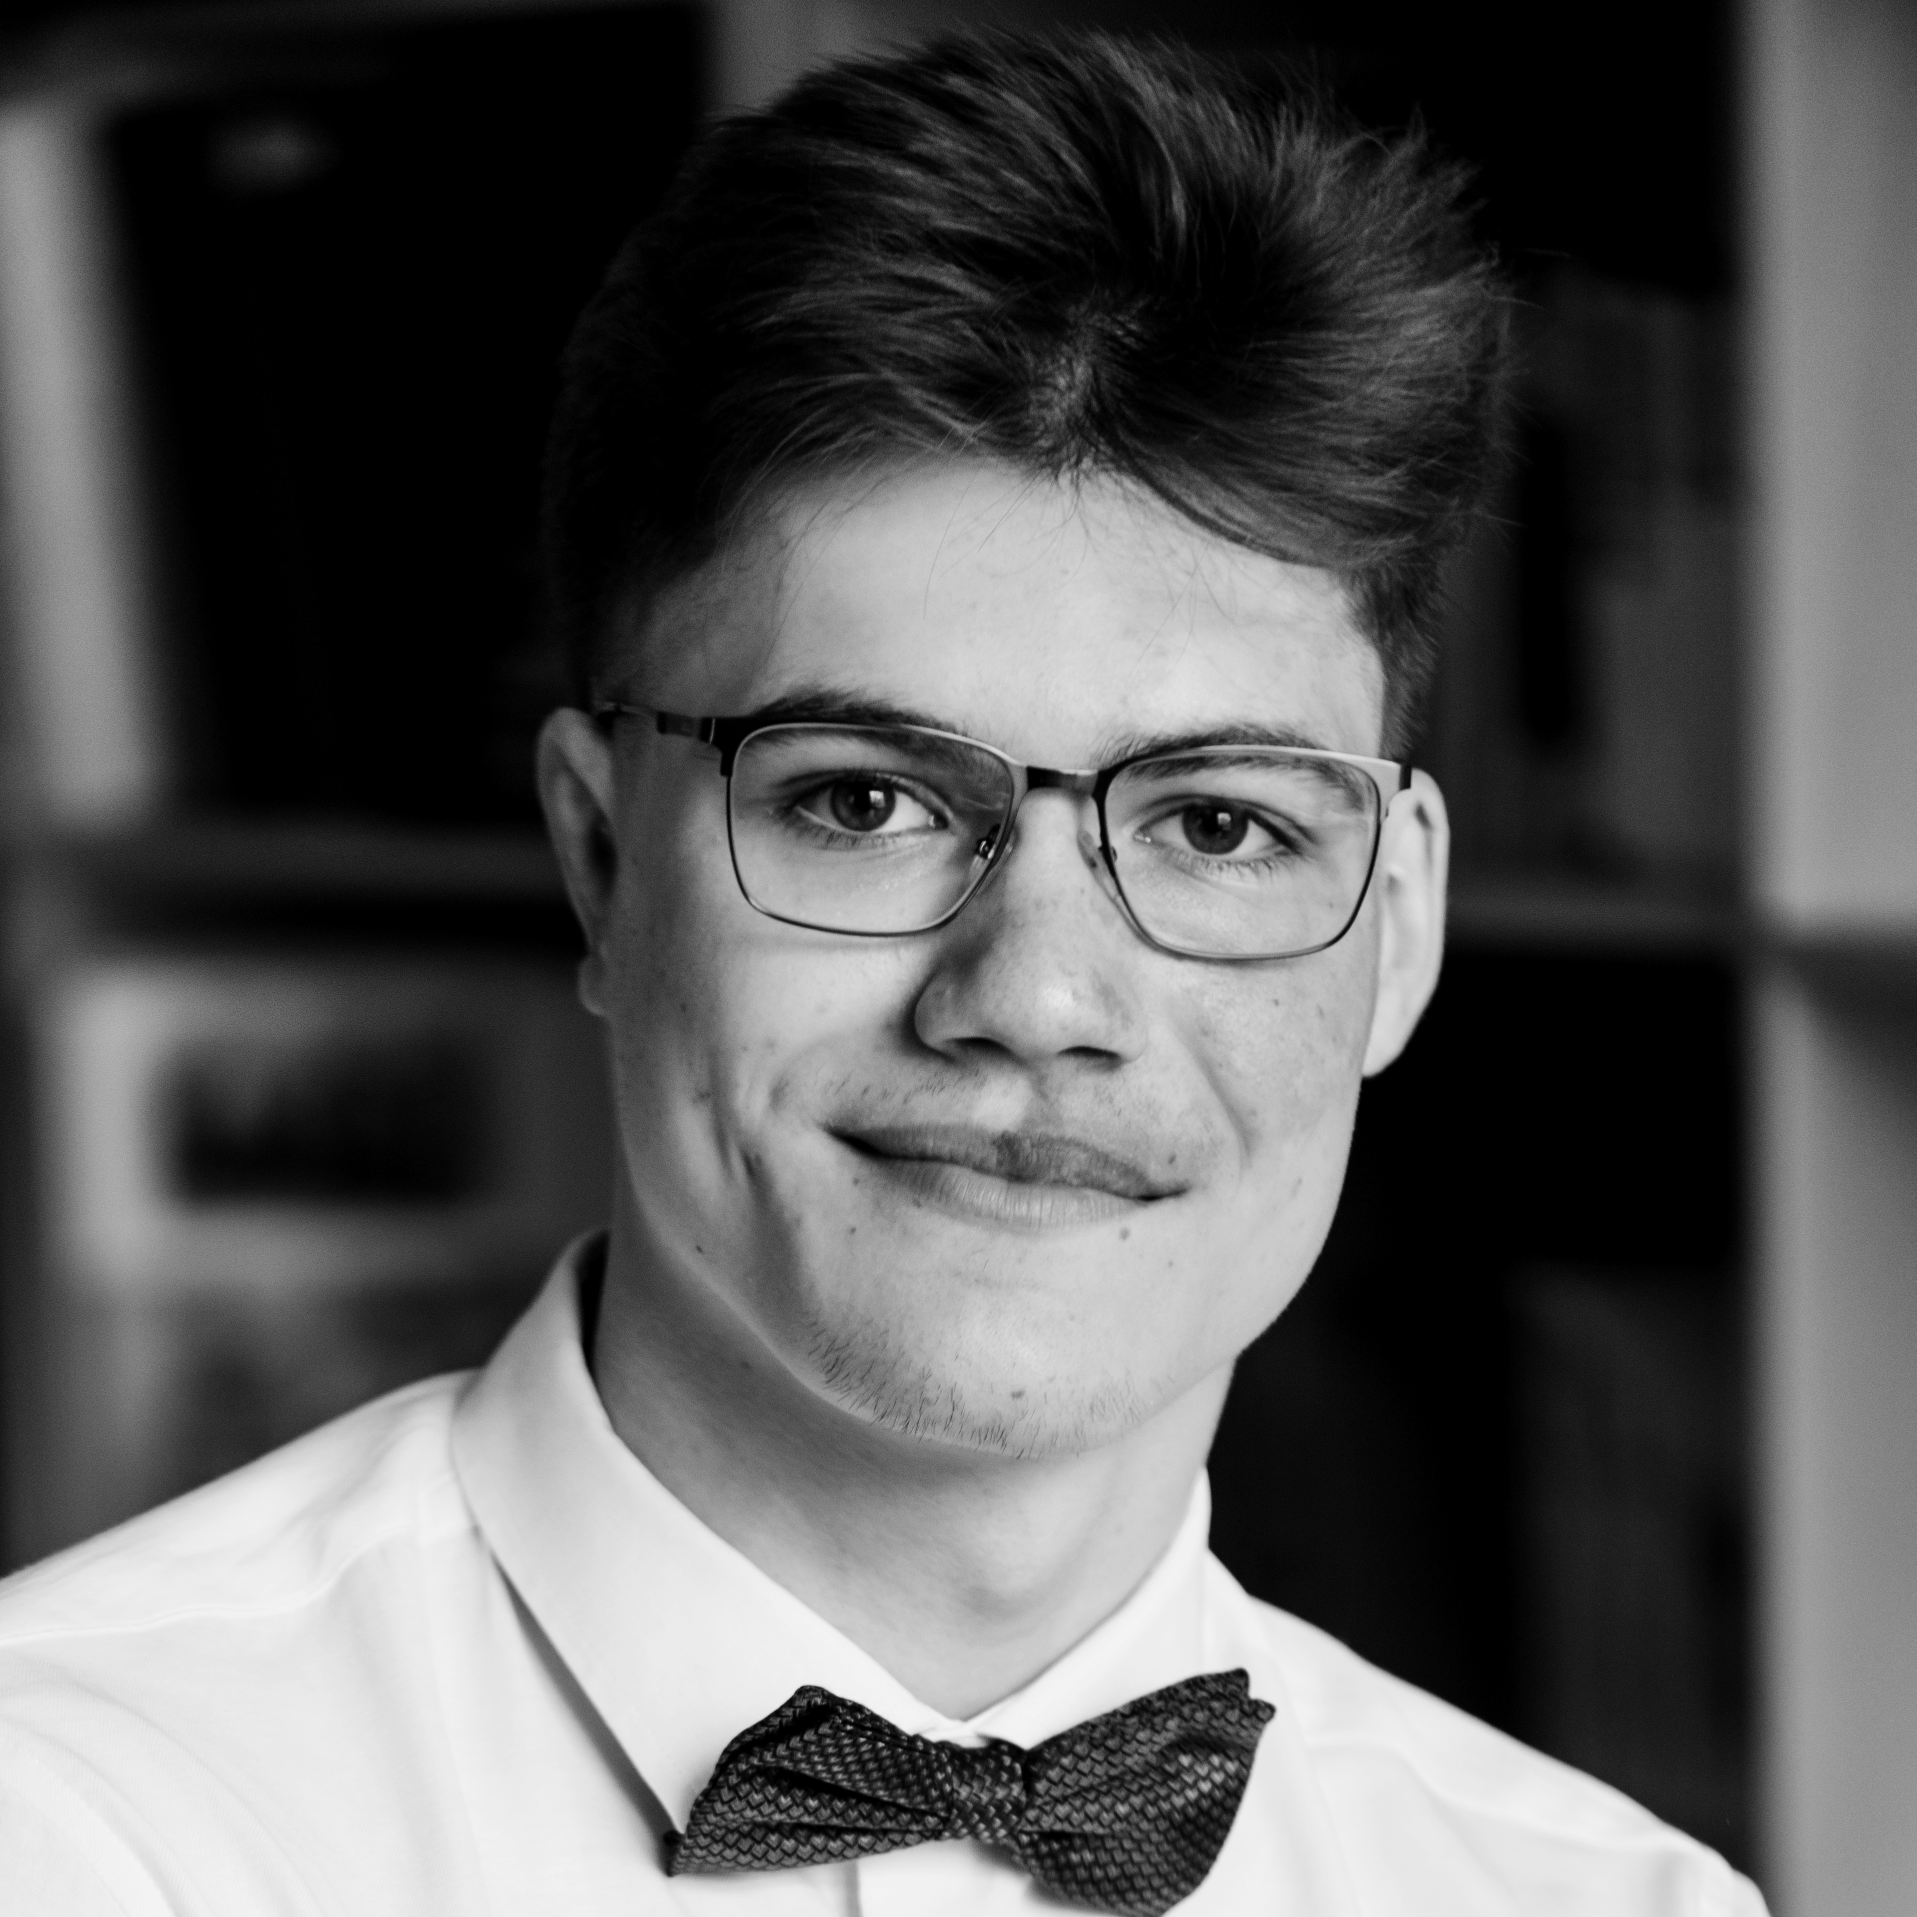
\includegraphics[width=4cm]{media/Photo.jpg}};
\end{tikzpicture}

\MySkip

{\LARGE \bfseries Andrey Karchevsky}
\MySkip
{\Large \bfseries \textcolor{ColorOne}{Data Engineer}}

\MySkip

\faMapPin\hspace{0.2em} Russia, Saint Petersburg \\
\faEnvelope\hspace{0.2em} \myhref{mailto:karych@karych.ru}{karych@karych.ru}

\end{center}

\begin{flushleft}
\section*{Education \& Achievements}
\begin{description}[font=\normalfont\color{ColorOne},leftmargin=0pt,labelwidth=0pt]
	\item[2023--2027] \textbf{Bachelor in Computer Science} \\
	\href{https://itmo.ru/}{ITMO} University, \href{https://fitp.itmo.ru/p/about-fitp/753}{Software Engineering}.

	\item[2023] \textbf{ITMO.STARS: \myhref{https://news.itmo.ru/en/education/students/news/13345/}{Winner}} \\
	ITMO.STARS is a \myhref{https://stars.itmo.ru/}{contest} for applicants with unique achievements. Winning this competition provides a grant for education at ITMO University.
\end{description}

\section*{Contacts \& \\ Resources}
\begin{description}[font=\normalfont\color{ColorOne},leftmargin=0pt,labelwidth=0pt]
    \item[\faGithub] \myhref{https://github.com/realkarych}{github.com/realkarych}
    \vspace{-0.5em}
    \item[\faTelegram] \myhref{https://t.me/karych}{t.me/karych}
    \vspace{-0.5em}
    \item[\faLinkedin] \myhref{https://www.linkedin.com/in/karych}{linkedin.com/in/karych
    \vspace{-0.5em}}
    \item[\faLink] \myhref{https://habr.com/ru/users/realkarych/}{habr.com/users/realkarych}
\end{description}
\end{flushleft}

\vfill
\end{minipage}
\end{adjustbox}
\hfill
% Vertical rule
\begin{adjustbox}{valign=t}
\begin{minipage}{0.02\textwidth}
\MyVerticalRule
\end{minipage}
\end{adjustbox}
\hfill
% Right column
\begin{adjustbox}{valign=t}
\begin{minipage}{0.65\textwidth}
\section*{A Little Bit About Myself}
\begin{flushleft}

\textbf{Data engineer} at \textbf{\href{https://codescoring.ru/}{CodeScoring}} \textit{(since November, 2024)}. Open-Source vulnerabilities domain.
Ensuring supply chains. Developing DWH: PostgreSQL, ClickHouse, Neo4j; data-pipelines on Apache Airflow.

\MySkip

Intern \textbf{data platform engineer} at \href{https://ya.ru}{\raisebox{-0.2em}{
\includegraphics[height=1em]{media/yandex.png}}~\hspace{-0.40em}\textbf{andex}} Search/Ads ML Infrastructure \textit{(May 2024 -- October 2024)}. Helped to develop platform for building data pipelines based on \href{https://github.com/ytsaurus/ytsaurus}{YTsaurus}. Implemented a new type of tasks (DAG nodes); upgraded AutoDoc -- a library for DAG nodes' dependencies codegen.

\MySkip

Author of \href{https://realkarych.github.io/rxconf/}{\raisebox{-0.35em}{
\includegraphics[height=1.4em]{media/rxconf.png}}\textbf{RxConf}}, a library for real-time configuration management in Python with built-in support for common config types.

\MySkip

Founder of \hspace{0.3em}\href{https://github.com/realkarych/postamt/}{\raisebox{-0.3em}{
\includegraphics[height=1.3em]{media/postamt_round.png}} \hspace{-0.1em}\textbf{Postamt}}, an experimental email client powered by Telegram forums and WebApps.

\MySkip

Maintainer of \hspace{0.2em}\href{https://github.com/realkarych/aioplate/}{\faGithub\hspace{0.1em}\textbf{Aioplate}}, a well-known template for building Telegram chatbots in Python using Aiogram.

\MySkip

Check out \textbf{over 10} other published projects on \href{https://github.com/realkarych}{my GitHub}. \\
\end{flushleft}

\section*{Current Stack}
\begin{tabular}{@{}p{5cm}p{9cm}@{}}
    \textbf{Python}                      & \textbf{3.x}, \textbf{2.x} \\
    \textbf{BigData \& ETL}              & \textbf{Apache Airflow}, \textbf{Spark} \\
    \textbf{Databases}                   & \textbf{PostgreSQL}, \textbf{ClickHouse}, \textbf{Neo4j} \\
    \textbf{ORMs}                        & \textbf{SQLAlchemy} \\
    \textbf{Python for Web}              & \textbf{FastAPI} \\
    \textbf{Data Validation}             & \textbf{Pydantic} as a hands-on tool \\
    \textbf{Containerization}            & \textbf{Docker}, \textbf{Docker Compose} \\
    \textbf{CI/CD}                       & \textbf{Actions}, release processes \\
    \textbf{Testing}                     & \textbf{PyTest}, the Testing Pyramid impl. \\
\end{tabular}
\end{minipage}
\end{adjustbox}
\end{document}
